\documentclass[../main.tex]{subfiles}

\begin{document}

\section*{第1問}

{\bf [解]}
\textbf{(1)} \underline{$1^\circ$ $0<a<1$}

$a^n\to0\ (n\to\infty)$から
\begin{align*}
(1+a^n)^{1/n}\longrightarrow1^0=1
\end{align*}

\underline{$2^\circ$ $a=1$}
\begin{align*}
(1+1)^{1/n}\longrightarrow1
\end{align*}

\underline{$3^\circ$ $1<a$}
\begin{align*}
(1+a^n)^{1/n}&=\left[a^n\left(1+\frac1{a^n}\right)\right]^{1/n}\\
&=a\sqrt[n]{1+\frac1{a^n}}\longrightarrow a
\end{align*}

以上から，
\begin{align*}
\lim_{n\to\infty}(1+a^n)^{1/n}=\begin{cases}1&(0<a\le1)\\a&(1<a)\end{cases}
\end{align*}

\textbf{(2)} $A=\displaystyle\int_1^{\sqrt3}\frac1{x^2}\log\sqrt{1+x^2}\,dx$とおく．
\begin{align*}
A&=\frac12\int_1^{\sqrt3}\frac1{x^2}\log(x^2+1)\,dx\\
&=\frac12\left[-\frac1x\log(x^2+1)\right]_1^{\sqrt3}+\frac12\int_1^{\sqrt3}\frac1x\cdot\frac{2x}{x^2+1}\,dx\\
&=-\frac12\left\{\frac1{\sqrt3}\log4-\log2\right\}+\int_1^{\sqrt3}\frac1{x^2+1}\,dx\\
&=-\frac12\left(\frac23\sqrt3-1\right)\log2+\Bigl[\arctan x\Bigr]_1^{\sqrt3}\\
&=\frac12\left(1-\frac23\sqrt3\right)\log2+\frac1{12}\pi．
\end{align*}

\bigskip
\noindent{\bf [解2]}
\textbf{(1)} \underline{$1^\circ$ $1<a$}

$a^n<1+a^n<2a^n$から，$a<\sqrt[n]{1+a^n}<2^{1/n}\cdot a$

\underline{$2^\circ$ $0<a\le1$}

$1<1+a^n\le2$から，$1<\sqrt[n]{1+a^n}<2^{1/n}$

ではさみうちの原理によりそれぞれの極限が定まる．（以下省略）

\newpage

\section*{第2問}

{\bf [解]}
点$X$に対し，$\overrightarrow{OX}=\vec x$とおく．正四面体$OABC$の一辺を$1$として良く，
\begin{align*}
\vec p=\alpha\vec a，\quad \vec q=\beta\vec b，\quad \vec r=\gamma\vec c\quad(0<\alpha,\beta,\gamma<1)
\end{align*}
とおく．$\overline{PQ}=\overline{QR}=\overline{RP}$から
\begin{align*}
|\alpha\vec a-\beta\vec b|^2=|\beta\vec b-\gamma\vec c|^2=|\gamma\vec c-\alpha\vec a|^2
\end{align*}

$|\vec a|=|\vec b|=|\vec c|=1$，$\vec a\cdot\vec b=\vec b\cdot\vec c=\vec c\cdot\vec a=\dfrac12$だから，$k>0$として
\begin{align*}
\alpha^2-\alpha\beta+\beta^2&=k\quad\cdots①\\
\beta^2-\beta\gamma+\gamma^2&=k\quad\cdots②\\
\gamma^2-\gamma\alpha+\alpha^2&=k\quad\cdots③
\end{align*}

①，②から
\begin{align*}
\alpha^2-\alpha\beta&=\gamma^2-\beta\gamma\\
(\alpha^2-\gamma^2)-\beta(\alpha-\gamma)&=0\\
(\alpha+\gamma-\beta)(\alpha-\gamma)&=0\quad\cdots④
\end{align*}

同様に
\begin{align*}
(\alpha+\beta-\gamma)(\alpha-\beta)&=0\quad\cdots⑤\\
(-\alpha+\beta+\gamma)(\beta-\gamma)&=0\quad\cdots⑥
\end{align*}

④から，$\alpha=\gamma$または$\beta=\alpha+\gamma$である．

\underline{$1^\circ$ $\alpha=\gamma$}

⑤，⑥から$\beta=\alpha=\gamma$であり，この時$AB\parallel PQ$，$BC\parallel QR$，$CA\parallel RP$が成り立つ（$\because$相似）．

\underline{$2^\circ$ $\beta=\alpha+\gamma$}

⑤に代入して，$(\alpha+\beta-\gamma)(\alpha-\beta)=(2\alpha)(-\gamma)=0$．$\alpha\ne0$だから$\gamma=0$となり，$0<\gamma<1$に矛盾する．

以上から示された．$\blacksquare$

\begin{figure}[htb]
\centering
\begin{tikzpicture}[scale=1.6, >=stealth]
  \coordinate (O) at (0,2.6);
  \coordinate (A) at (-2,0);
  \coordinate (B) at (2,0);
  \coordinate (C) at (0,-1);
  \coordinate (P) at ($(O)!0.55!(A)$);
  \coordinate (Q) at ($(O)!0.55!(B)$);
  \coordinate (R) at ($(O)!0.55!(C)$);
  \draw (O) -- (A) -- (B) -- cycle;
  \draw (O) -- (B);
  \draw (O) -- (C);
  \draw[dashed] (A) -- (C);
  \draw[dashed] (B) -- (C);
  \draw[thick] (P) -- (Q) -- (R) -- cycle;
  \node[above] at (O) {$O$};
  \node[left] at (A) {$A$};
  \node[right] at (B) {$B$};
  \node[below] at (C) {$C$};
  \node[left] at (P) {$P$};
  \node[right] at (Q) {$Q$};
  \node[below right] at (R) {$R$};
  \fill (P) circle (0.8pt);
  \fill (Q) circle (0.8pt);
  \fill (R) circle (0.8pt);
\end{tikzpicture}
\caption{正四面体$OABC$と辺上の点$P$，$Q$，$R$}
\end{figure}

\newpage

\section*{第3問}

{\bf [解]}
$\alpha=x+y$，$\beta=xy$とおくと，題意及び$x,y$の実数条件から，
\begin{align*}
\alpha^2-4\beta&\ge0\quad\cdots①\\
\alpha^2-\beta&=6\quad\cdots②
\end{align*}

又，与式を$f(\alpha,\beta)$とすると
\begin{align*}
f(\alpha,\beta)&=xy(x+y)-(x+y)^2+(x+y)\\
&=\beta\alpha-\alpha^2+\alpha\quad\cdots③
\end{align*}

となる．②から$\beta=\alpha^2-6$だから①，③に代入して
\begin{align*}
\alpha^2-4(\alpha^2-6)&\ge0\\
f(\alpha,\beta)&=\alpha^3-\alpha^2-5\alpha
\end{align*}

第1式から，$-2\sqrt2\le\alpha\le2\sqrt2\quad\cdots④$である．
\begin{align*}
\frac{d}{d\alpha}f=3\alpha^2-2\alpha-5=(3\alpha-5)(\alpha+1)
\end{align*}

よって下表を得る．

\begin{center}
\begin{tabular}{c|ccccccc}
$\alpha$ & $-2\sqrt2$ & & $-1$ & & $5/3$ & & $2\sqrt2$ \\
\hline
$f'$ & & $+$ & $0$ & $-$ & $0$ & $+$ & \\
\hline
$f$ & $-6\sqrt2-8$ & $\nearrow$ & $3$ & $\searrow$ & $-\dfrac{175}{27}$ & $\nearrow$ & $6\sqrt2-8$ \\
\end{tabular}
\end{center}

よって，$3>6\sqrt2-8$及び$-6\sqrt2-8<-\dfrac{175}{27}$から
\begin{align*}
-2(3\sqrt2+4)\le f\le3．
\end{align*}

\newpage

\section*{第4問}

{\bf [解]}
\textbf{(1)} $\sqrt[3]2$が有理数だとする．この時$a\in\mathbb N$，$b\in\mathbb N$，$a\perp b$として
\begin{align*}
\sqrt[3]2=\frac ba\quad\therefore\ 2a^3=b^3
\end{align*}
とかける．したがって$b^3$が$2$の因数を持ち，$2$は素数だから$b$は$2$の倍数．この時$b=2b'\ (b'\in\mathbb N)$とかけるから
\begin{align*}
a^3=4b'^3
\end{align*}
となり同じく$a$も$2$の倍数となり，$a\perp b$に反する．よって矛盾し，$\sqrt[3]2\notin\mathbb Q$．$\blacksquare$

\textbf{(2)} $\alpha=\sqrt[3]2$とおく．$Q(x)$を有理数係数の整式として
\begin{align*}
P(x)=Q(x)(x^3-2)+ax^2+bx+c\quad\cdots\text{※}
\end{align*}
とおける．ただし，$a,b,c\in\mathbb{Q}$である．$P(\alpha)=0$から
\begin{align*}
a\alpha^2+b\alpha+c=0\quad\cdots①
\end{align*}

ここで，$a=0$の時，$b=c=0$ならOKだが，その他の場合は（1)から）$\alpha$が$b,c\in\mathbb Q$を用いて有理数と表せることになり矛盾．$\quad\cdots②$

又，$a\ne0$の時，$x^3-2$を$R(x)=ax^2+bx+c$で割った商$S(x)$，あまり$T(x)$として
\begin{align*}
x^3-2=R(x)S(x)+T(x)\quad\cdots\text{※}
\end{align*}
ただし$T(x)$は1次以下の整式で，$x=\alpha$として
\begin{align*}
T(\alpha)=0
\end{align*}
だが，これは上記の$a=0$の場合と同様にして，$T(x)\equiv0$となる．よって
\begin{align*}
x^3-2=R(x)S(x)=(x^2+\alpha x+\alpha^2)(x-\alpha)
\end{align*}
で$R(x)$が2次式だから
\begin{align*}
R(x)=x^2+\alpha x+\alpha^2
\end{align*}
となり，$R(x)$の係数が有理数であることに反し矛盾．$\quad\cdots③$

②③から，$a=b=c=0$で，この時$P(x)$は$x^3-2$で割り切れる．$\blacksquare$

\bigskip
\noindent{\bf [解2]}
（前略）
\begin{align*}
a\alpha^2+b\alpha+c=0\quad\cdots④
\end{align*}
両辺に$\alpha$をかけて，$\alpha^3=2$から
\begin{align*}
b\alpha^2+c\alpha+2a=0\quad\cdots⑤
\end{align*}

④$\times b$－⑤$\times a$より
\begin{align*}
(b^2-ac)\alpha+bc-2a^2=0
\end{align*}

$\alpha\notin\mathbb Q$だから
\begin{align*}
b^2-ac=0，\qquad bc-2a^2=0
\end{align*}

ここで，$c$を消去して，$a\ne0$とすると
\begin{align*}
b^3=2a^3\quad\therefore\ \alpha=\frac ba
\end{align*}
から，$\alpha\in\mathbb Q$に反し矛盾．よって$a=b=c=0$となり，示された．$\blacksquare$

\newpage

\section*{第5問}

{\bf [解]}
\textbf{(p)} 正$n$角形の頂点を左から$A_1,\ldots,A_n$とする．$\angle A_lA_2A_m$（$l<m$）が$60^\circ$に等しい時，正$n$角形は円に内接することと円周角の定理から，$l=2$の時を考えれば良い．正$n$角形の内接する円の中心を$O$とし，この半径を$1$として良い．$\triangle A_1A_2A_m$に正弦定理を用いて，
\begin{align*}
\frac{\overline{A_1A_m}}{\sin60^\circ}=2\quad\therefore\ \overline{A_1A_m}=\sqrt3\quad\cdots①
\end{align*}

一方，$\angle A_1OA_m=2\pi\dfrac{n-m+1}n$だから，
\begin{align*}
\overline{A_1A_m}=2\sin\pi\frac{n-m+1}n\quad\cdots②
\end{align*}

①，②から
\begin{align*}
\sin\frac{n-m+1}n\pi&=\frac{\sqrt3}2\\
\sin\left(\pi-\frac{m-1}n\pi\right)&=\frac{\sqrt3}2\\
\sin\frac{m-1}n\pi&=\frac{\sqrt3}2
\end{align*}

$3\le m\le n$から，$0<\dfrac{m-1}n<1$だから，
\begin{align*}
\frac{m-1}n\pi=\frac13\pi,\ \frac23\pi
\end{align*}
\begin{align*}
n=3(m-1)\quad\text{or}\quad n=3\cdot\frac{m-1}2
\end{align*}

$m\in\mathbb N$及びいずれの場合も，$n$は$3$の倍数である．よって(p)は正しい．

\textbf{(q)} 下図のような正六角形内に$A$，$B$，$C$，$D$をとる．この時，(p)の議論から，
\begin{align*}
\angle ACB=\angle ADB\quad\cdots③
\end{align*}
であり，かつ
\begin{align*}
\overline{AC}<\overline{AD}，\quad\overline{BC}<\overline{BD}\quad\cdots④
\end{align*}
となる．したがって，③，④から，このような4点$A,B,C,D$は(q)の反例となる．よって(q)は正しくない．

\begin{figure}[htb]
\centering
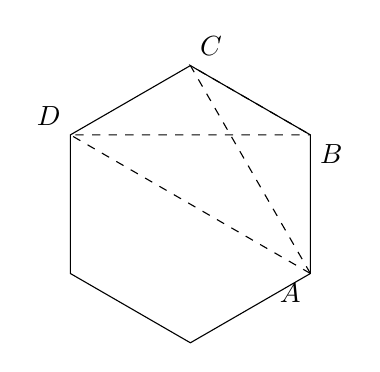
\begin{tikzpicture}[scale=1.1, >=stealth]
  \foreach \i in {0,...,5} {
    \coordinate (V\i) at ({90+60*\i}:1.6);
  }
  \draw (V0) -- (V1) -- (V2) -- (V3) -- (V4) -- (V5) -- cycle;
  \node[above right] at (V0) {$C$};
  \node[above left] at (V1) {$D$};
  \node[below left] at (V4) {$A$};
  \node[below right] at (V5) {$B$};
  \draw[dashed] (V4) -- (V0) -- (V5);
  \draw[dashed] (V4) -- (V1) -- (V5);
\end{tikzpicture}
\caption{正六角形内の点$A$，$B$，$C$，$D$（(q)の反例）}
\end{figure}

\newpage

\section*{第6問}

{\bf [解]}
$\dfrac{1+\sqrt3}2\le Y_{n+1}\le1+\sqrt3$となる時，これを整理すると
\begin{align*}
\frac{1+\sqrt3}2-X_{n+1}\le\frac1{Y_n}\le1+\sqrt3-X_{n+1}\quad\cdots①
\end{align*}
となる．$\dfrac1{Y_n}>0$から，右側の不等式より，$1+\sqrt3-X_{n+1}>0\ \therefore X_{n+1}=1,2$が必要．また，$Y_1=X_1$も条件をみたすことから，$X_1=1,2$．以上あわせて，帰納的に$X_n=1,2$となる．この時，$X_{n+1}$で場合分け．

\underline{$1^\circ$ $X_{n+1}=1$}

①から
\begin{align*}
\frac{1+\sqrt3}2-1\le\frac1{Y_n}\le1+\sqrt3-1
\end{align*}
\begin{align*}
\frac{\sqrt3}3\le Y_n\le1+\sqrt3
\end{align*}
ならば良い．

\underline{$2^\circ$ $X_{n+1}=2$}

①から
\begin{align*}
\frac{1+\sqrt3}2-2\le\frac1{Y_n}\le1+\sqrt3-2
\end{align*}
\begin{align*}
\frac{1+\sqrt3}2\le Y_n
\end{align*}

だから，①となる時
\begin{align*}
&\frac{\sqrt3}3\le Y_n<\frac{1+\sqrt3}2\ \text{の時，}X_{n+1}=1，\\
&\frac{1+\sqrt3}2\le Y_n\le1+\sqrt3\ \text{の時，}X_{n+1}=1\ \text{or}\ 2，\\
&1+\sqrt3<Y_n\ \text{の時，}X_{n+1}=2
\end{align*}
である．ここで，$Y_1\ge1$と$X_n\ge1$より帰納的に$Y_n\ge1$であることから，
\begin{align*}
p_{n+1}&=\frac26p_n+\frac16(1-p_n)\\
&=\frac16p_n+\frac16
\end{align*}

ここで，$p_1=\dfrac16$だから，
\begin{align*}
p_n=\frac15\left\{1-\left(\frac16\right)^n\right\}．
\end{align*}

\newpage

\end{document}
